%%%%%%%%%%%%%%%%%%%%%%%%%%%%%%%%%%%%%%%%%
% Beamer Presentation
% LaTeX Template
% Version 1.0 (10/11/12)
%
% This template has been downloaded from:
% http://www.LaTeXTemplates.com
%
% License:
% CC BY-NC-SA 3.0 (http://creativecommons.org/licenses/by-nc-sa/3.0/)
%
%%%%%%%%%%%%%%%%%%%%%%%%%%%%%%%%%%%%%%%%%

%----------------------------------------------------------------------------------------
%	PACKAGES AND THEMES
%----------------------------------------------------------------------------------------

\documentclass[mathserif]{beamer}

%% Použité kódování znaků: obvykle latin2, cp1250 nebo utf8:
\usepackage[utf8]{inputenc}

\mode<presentation> {

% The Beamer class comes with a number of default slide themes
% which change the colors and layouts of slides. Below this is a list
% of all the themes, uncomment each in turn to see what they look like.

%\usetheme{default}
%%\usetheme{AnnArbor}
%\usetheme{Antibes}
%\usetheme{Bergen}
%\usetheme{Berkeley} % 9
%\usetheme{Berlin}
%\usetheme{Boadilla}
%\usetheme{CambridgeUS}
%\usetheme{Copenhagen}
%\usetheme{Darmstadt}
%\usetheme{Dresden}
%\usetheme{Frankfurt}
%\usetheme{Goettingen}
%\usetheme{Hannover} % 8
%\usetheme{Ilmenau}
%\usetheme{JuanLesPins}
%\usetheme{Luebeck}
%%\usetheme{Madrid}
%\usetheme{Malmoe}
\usetheme{Marburg} % 8.5
%\usetheme{Montpellier}
%\usetheme{PaloAlto}
%\usetheme{Pittsburgh}
%\usetheme{Rochester}
%\usetheme{Singapore}
%\usetheme{Szeged}
%\usetheme{Warsaw}

% As well as themes, the Beamer class has a number of color themes
% for any slide theme. Uncomment each of these in turn to see how it
% changes the colors of your current slide theme.

%\usecolortheme{albatross}
%\usecolortheme{beaver} % 7.5
%\usecolortheme{beetle}
%\usecolortheme{crane}
%\usecolortheme{dolphin}
%\usecolortheme{dove}
%\usecolortheme{fly}
%\usecolortheme{lily}
%\usecolortheme{orchid}
%\usecolortheme{rose}
%\usecolortheme{seagull}
\usecolortheme{seahorse} % 7.5
%\usecolortheme{whale}
%\usecolortheme{wolverine}

%\setbeamertemplate{footline} % To remove the footer line in all slides uncomment this line
%\setbeamertemplate{footline}[page number] % To replace the footer line in all slides with a simple slide count uncomment this line

%\setbeamertemplate{navigation symbols}{} % To remove the navigation symbols from the bottom of all slides uncomment this line
}

\setbeamertemplate{blocks}[rounded][shadow=true]

\setbeamercolor{section in sidebar}{fg=yellow}
\setbeamercolor{subsection in sidebar}{fg=yellow}
\setbeamercolor{author in sidebar}{fg=green}
\setbeamercolor{block body}{bg=normal text.bg!90!black}
\setbeamercolor{block title}{bg=blue,fg=white}
\setbeamercolor{block body example}{bg=normal text.bg!90!black}
\setbeamercolor{block title example}{bg=black,fg=white}
\setbeamercolor{block body alerted}{bg=normal text.bg!90!black}
\setbeamercolor{block title alerted}{bg=red,fg=white}

\usepackage{graphicx} % Allows including images
\usepackage{booktabs} % Allows the use of \toprule, \midrule and \bottomrule in tables

\newtheorem{thm}{Věta}[section]
\newtheorem{lem}[thm]{Lemma}
\newtheorem{prop}[thm]{Tvrzení}

%----------------------------------------------------------------------------------------
%	TITLE PAGE
%----------------------------------------------------------------------------------------

\title[Oddělovací axiomy]{Oddělovací axiomy v bezbodové topologii} % The short title appears at the bottom of every slide, the full title is only on the title page

\author{Karel Ha} % Your name
\institute[MFF UK] % Your institution as it will appear on the bottom of every slide, may be shorthand to save space
{
Matematicko-fyzikální fakulta, \\
Univerzita Karlova v Praze \\ % Your institution for the title page
}
\titlegraphic{%
  \begin{columns}[r]
    \begin{column}[R]{.5\textwidth} % each column can also be its own environment
      \includegraphics[height=3.6cm]{img/logo_UK.jpg}
    \end{column}
    \begin{column}[R]{.5\textwidth} % alternative top-align that's better for graphics
      \includegraphics[height=3cm]{img/logo.pdf}
    \end{column}
  \end{columns}
}
\date{20. června 2013} % Date, can be changed to a custom date

\begin{document}

\begin{frame}
\titlepage % Print the title page as the first slide
\end{frame}

%\begin{frame}
%\frametitle{Přehled} % Table of contents slide, comment this block out to remove it
%\tableofcontents % Throughout your presentation, if you choose to use \section{} and \subsection{} commands, these will automatically be printed on this slide as an overview of your presentation
%\end{frame}

%----------------------------------------------------------------------------------------
%	PRESENTATION SLIDES
%----------------------------------------------------------------------------------------

%------------------------------------------------
\section{Úvod} % Sections can be created in order to organize your presentation into discrete blocks, all sections and subsections are automatically printed in the table of contents as an overview of the talk
%------------------------------------------------

\subsection{Klasický případ}

\begin{frame}
\frametitle{Klasický případ}
\framesubtitle{v bodové topologii}
\pause

{\color{blue}{Oddělovací axiomy} $T_i$} (pro $i = 0, 1, 2, 3, 3\frac{1}{2}, 4$)
se týkají oddělování:
\pause

\begin{itemize}[<+->]
  \item bodů od jiných bodů
  \item bodů od uzavřených množin
  \item uzavřených množin od jiných uzavřených množin
\end{itemize}

\uncover<6->{
  \begin{block}{Vztahy v~klasické topologii}
    \begin{align*}
      (T_4) \& (T_1)
             &\; \Longrightarrow \; (T_{3\frac{1}{2}}) \& (T_1)
    \; \Longrightarrow \; (T_3) \& (T_1)
      \; \Longrightarrow \; \\
      &\; \Longrightarrow \; (T_2)
      \; \Longrightarrow \; (T_1)
      \; \Longrightarrow \; (T_0)
    \end{align*}
    \pause
    \alert{Přídání axiomu $(T_1)$ u~třetí implikace je nezbytné!}
  \end{block}
}
\end{frame}

%------------------------------------------------

\subsection{Definice ``frame''}

\begin{frame}
\frametitle{Co je to ``frame''?}
Bezbodový přístup: místo~bodů pouze \alert{otevřené množiny}
\pause

\begin{block}{Definice}
  {\color{blue}Frame} je úplný svaz $L$ splňující
  \begin{equation*}% \tag{Frm}
    a \wedge \bigvee B
    = \bigvee \left\{ a \wedge b \mid b \in B \right\}
  \end{equation*}
  pro $a \in L$ a $B \subseteq L$.
\end{block}
\pause

\begin{exampleblock}{Příklad}
  Svaz otevřených množin dané topologie tvoří frame.
\end{exampleblock}
\end{frame}

%------------------------------------------------
\section{Axiomy oddělování}
%------------------------------------------------

\subsection{$T_0$} % A subsection can be created just before a set of slides with a common theme to further break down your presentation into chunks

\begin{frame}
\frametitle{Axiom $T_0$}

\begin{block}{Definice $(T_0)$}
  Pro každá $x \ne y$ existuje otevřená množina $U$ taková, že $x \in U
  \not\owns y$ nebo $x \not\in U \ni y$.
\end{block}

\begin{center}
  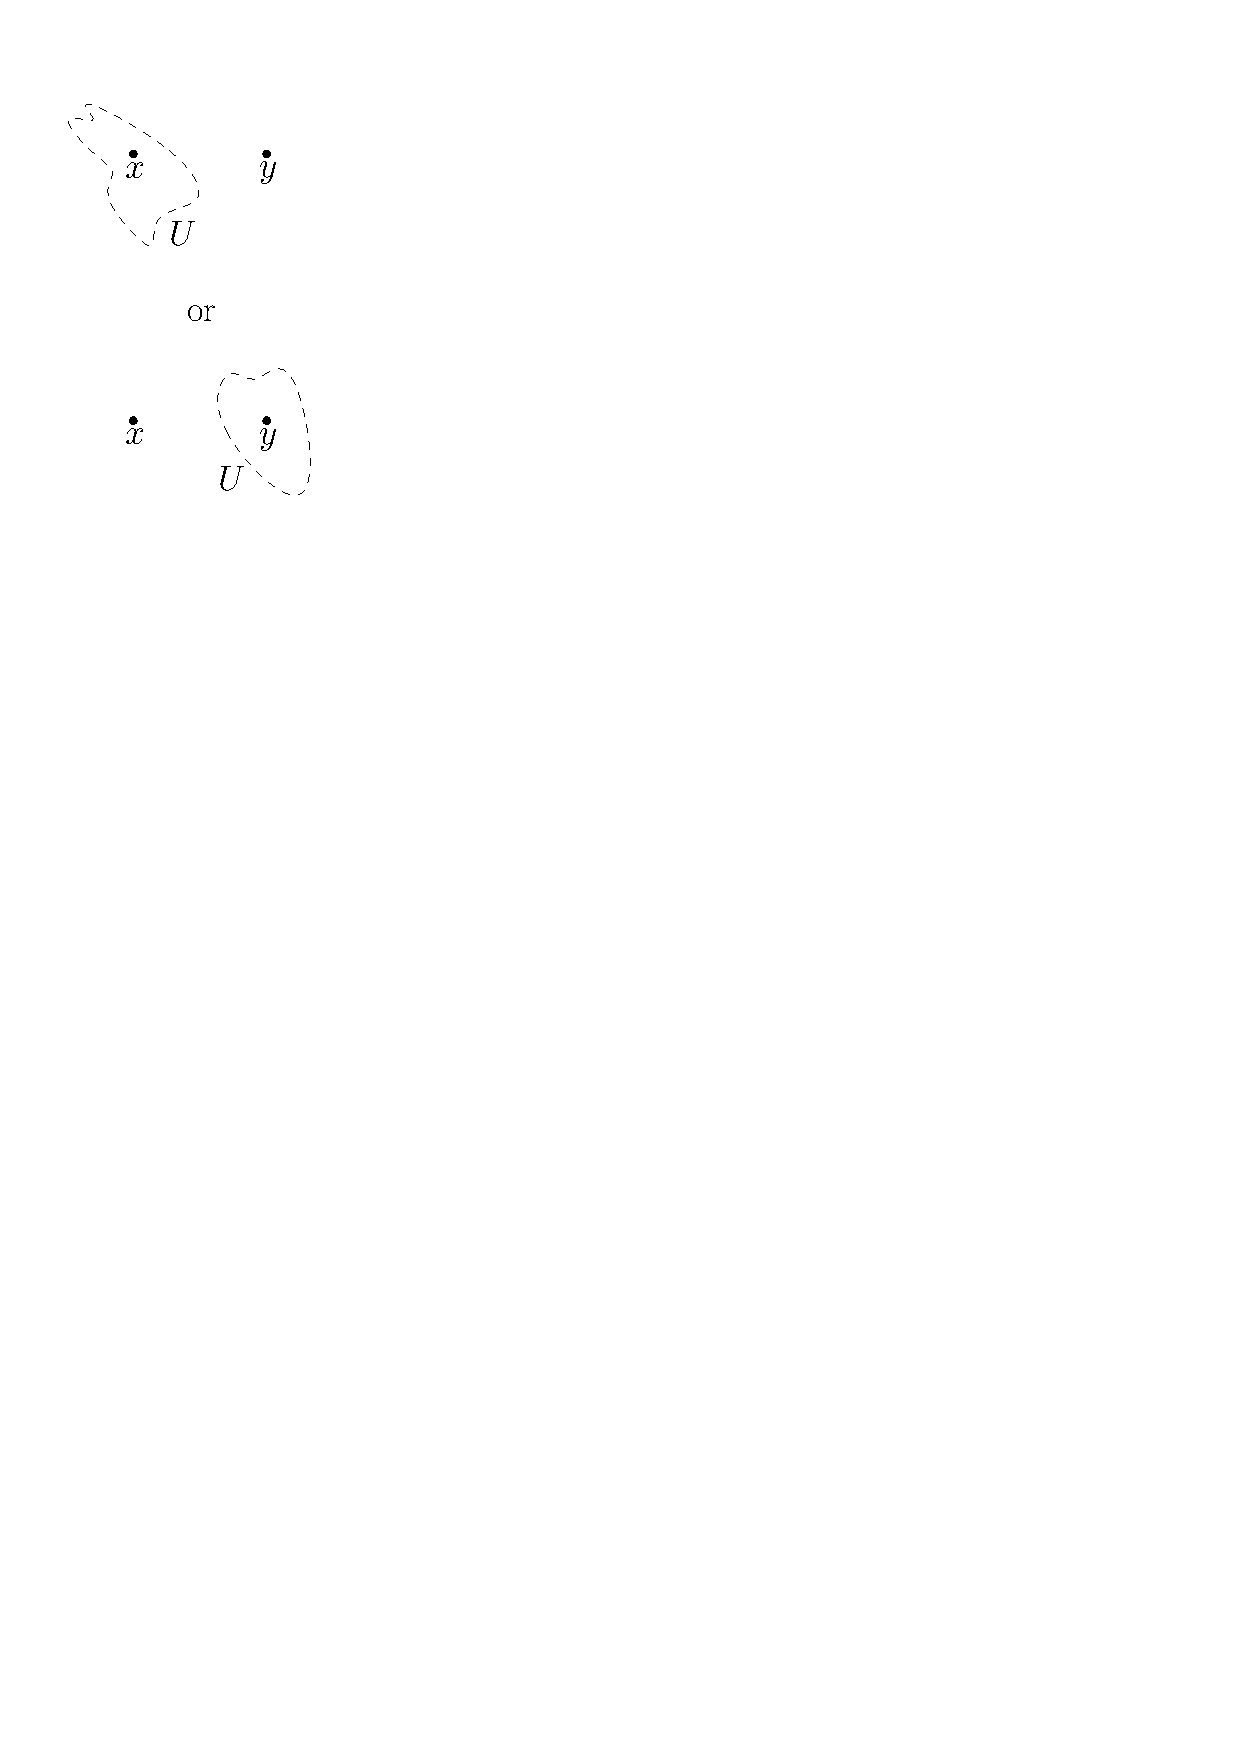
\includegraphics[height=3.3cm]{img/t0.pdf}
\end{center}
\pause

Předpokládejme, že je \alert{vždy splňen}.

(Ztotožnění bodů nerozlišitelných otevřenými množinami.)

\end{frame}

%------------------------------------------------

\subsection{Subfitness}

\begin{frame}
\frametitle{Subfitness}

\begin{block}{Definice $(T_1)$}
  Pro každá $x \ne y$ existuje otevřená množina $U_x$ taková, že $x \in U_x
  \not\owns y$.
\end{block}

\begin{center}
  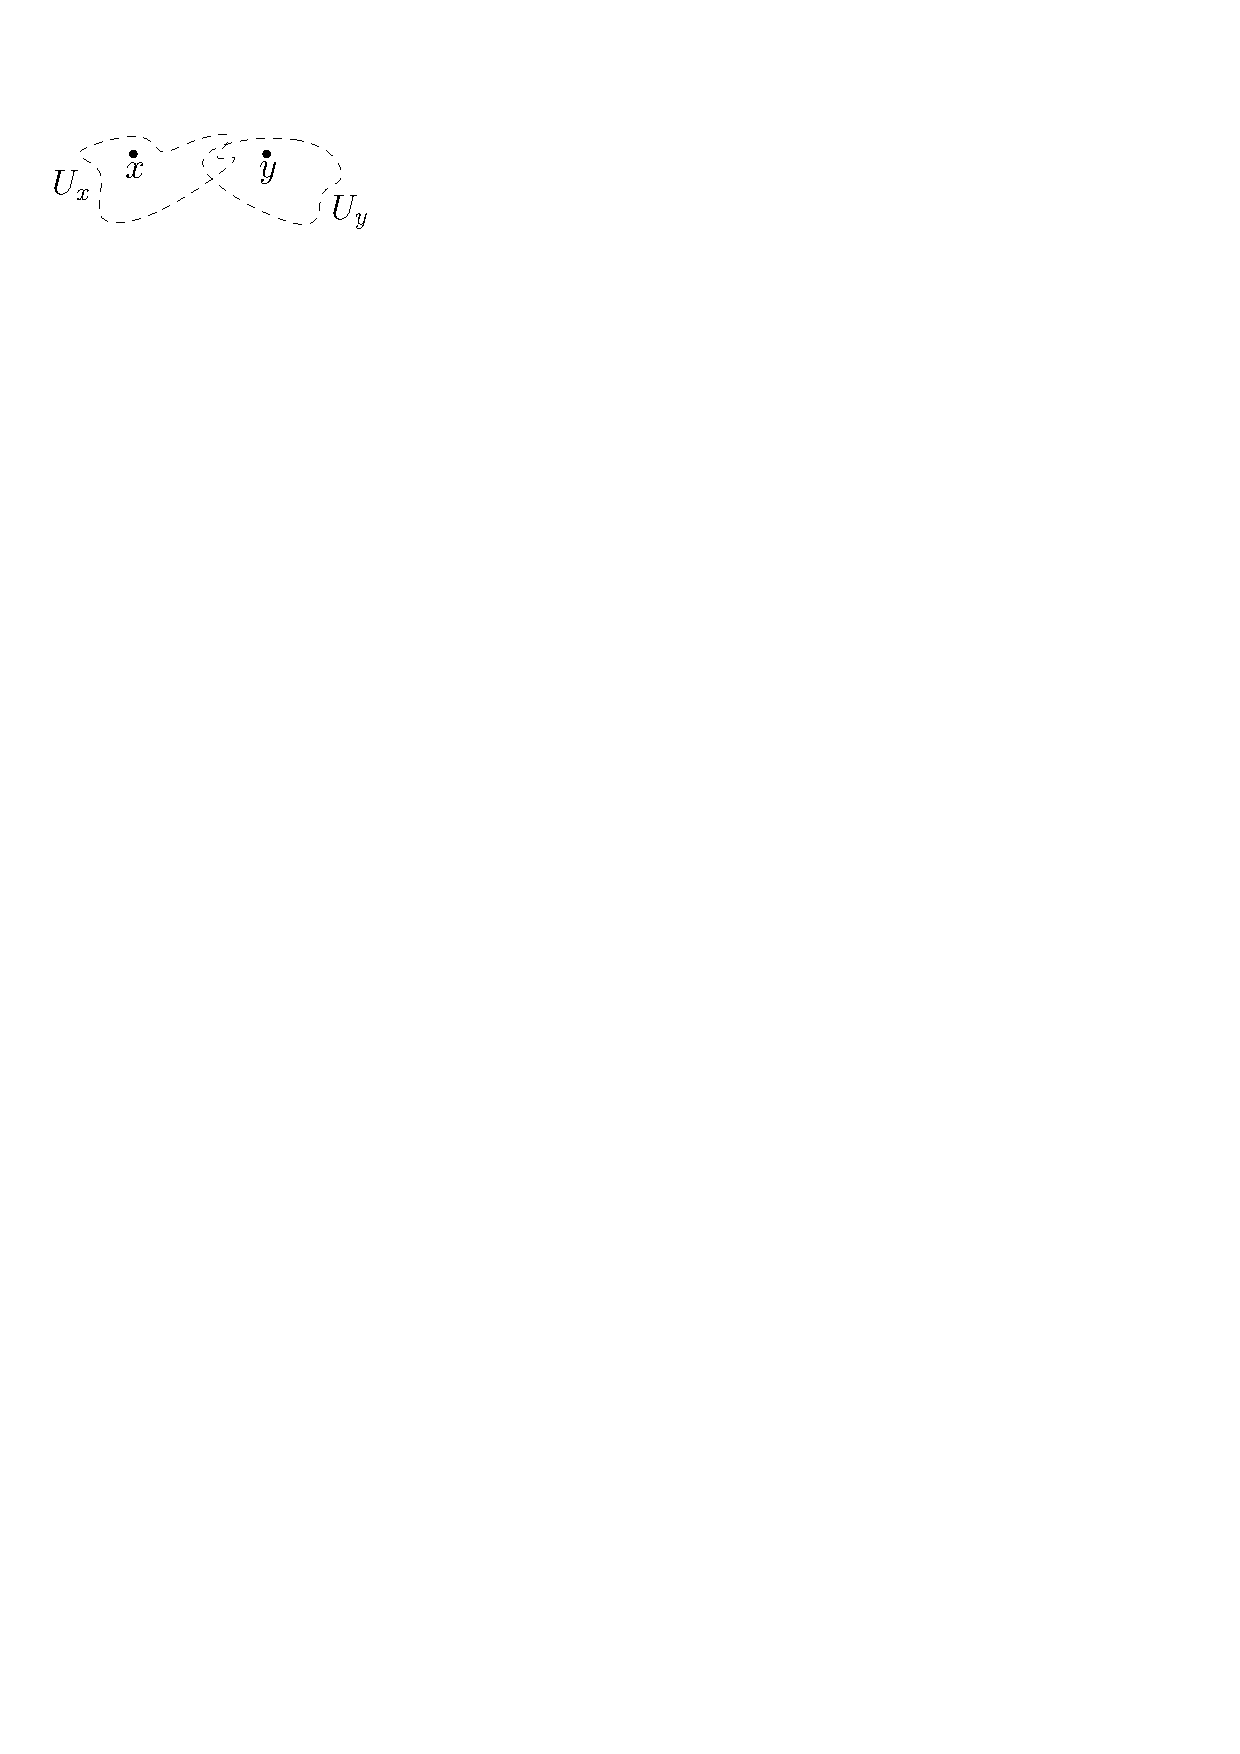
\includegraphics[width=.4\textwidth]{img/t1.pdf}
\end{center}
\pause

\begin{block}{Definice \textit{(Sfit)}}
  \[
    a \not\le b \qquad \Rightarrow \qquad \exists c, \quad a \vee c = 1 \ne b
    \vee c
  \]
\end{block}
\pause

Slabší vlastnost: \alert{$(T_1) \Rightarrow \textit{(Sfit)}$.}
\end{frame}

%------------------------------------------------

\subsection{Hausdorffova vlastnost}

\begin{frame}
\frametitle{Hausdorffův axiom}

\begin{block}{Definice $(T_2)$}
  Pro každá $x \ne y$ existují \alert{disjunktní} otevřené množiny $U, V$
  takové, že $x \in U, y \in V$.
\end{block}

\begin{center}
  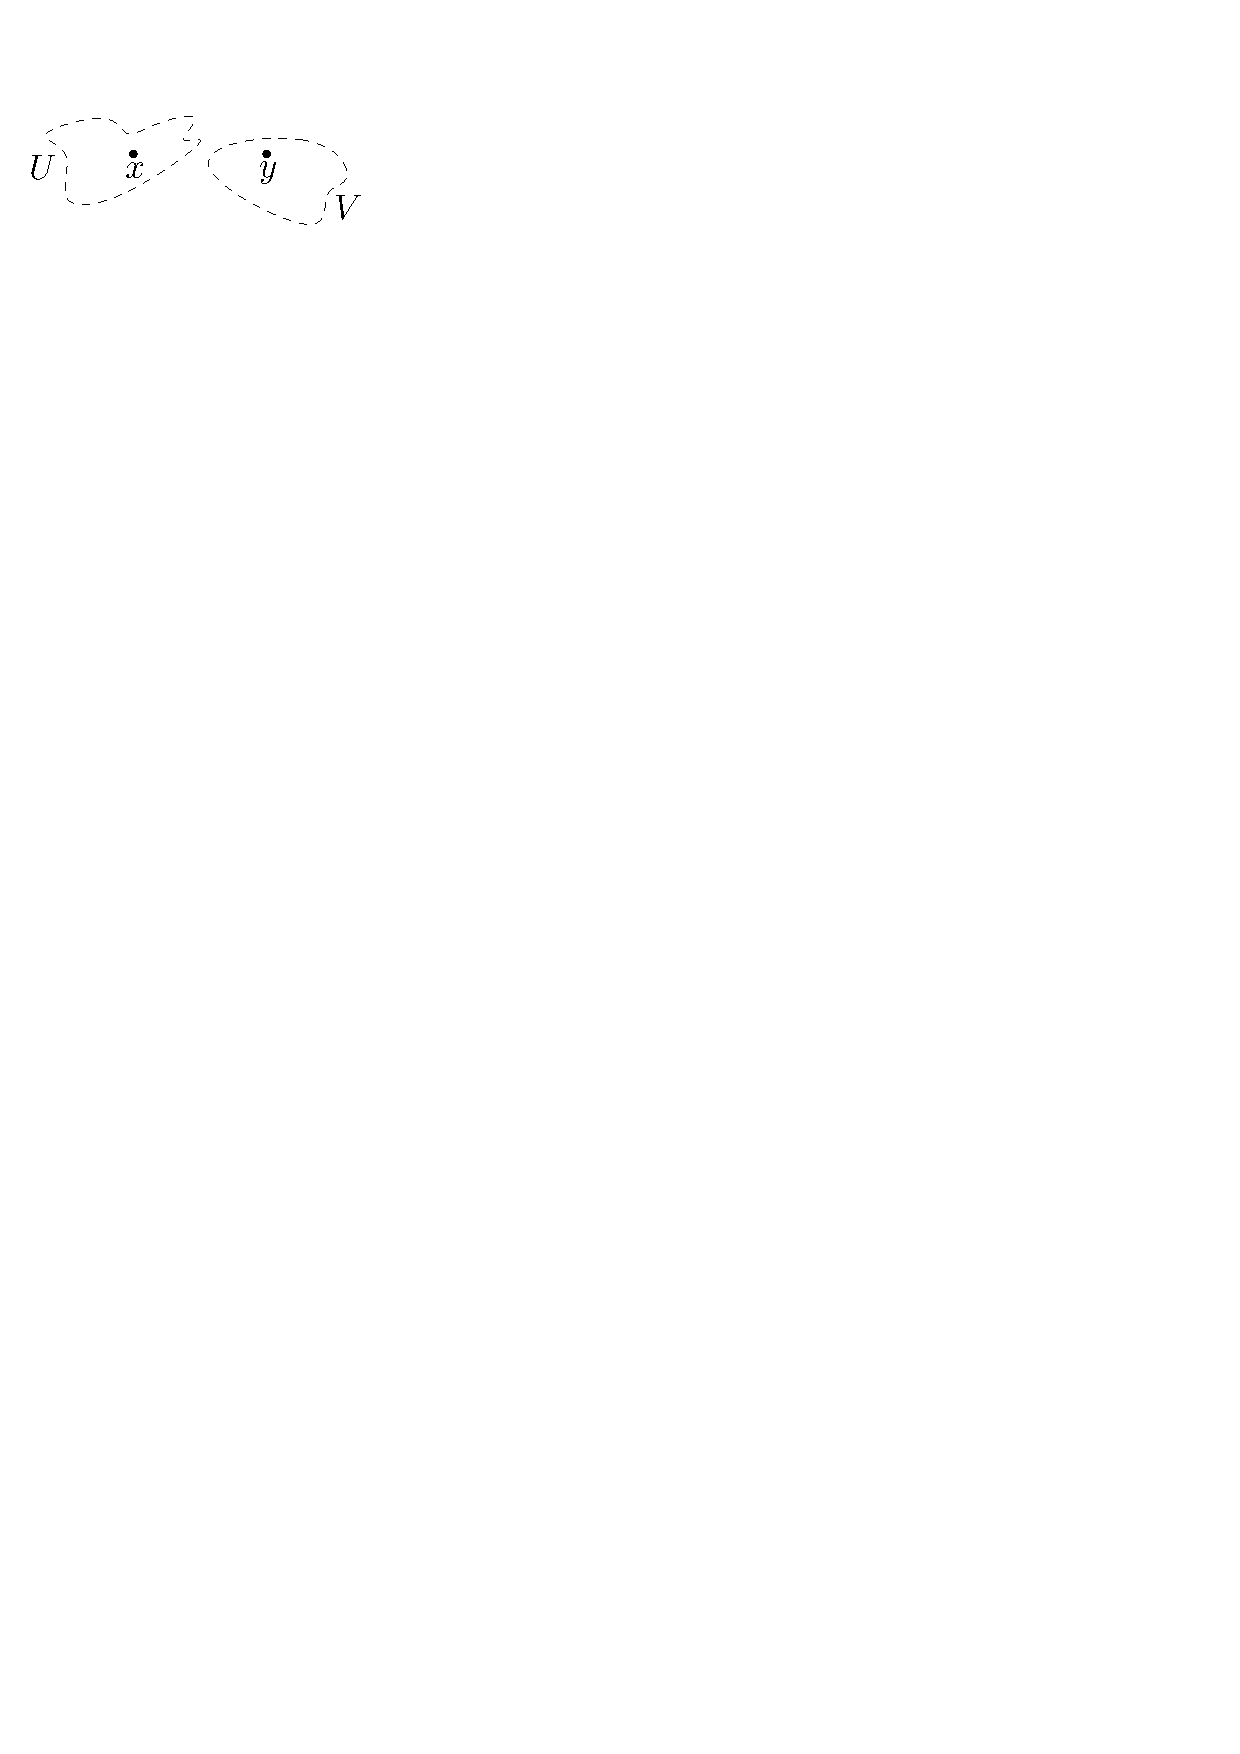
\includegraphics[width=.4\textwidth]{img/t2.pdf}
\end{center}
\pause

V bezbodové topologii je několik alternativ...
\end{frame}

%------------------------------------------------

\begin{frame}
\frametitle{Axiomy Hausdorffova typu}

Dowker-Straussův přístup:
\pause
\begin{block}{Definice \textit{(DS-Haus)}}
  \begin{center}
    $a \not\le b, a \not\ge b \qquad \Rightarrow \qquad \exists u\not\leq a,
    v\not\leq b, \quad u \wedge v = 0$
  \end{center}
\end{block}
\pause

Isbellův přístup:
\pause
\newcommand{\dL}{\, \uparrow \Delta(0)}
\begin{block}{Definice \textit{(I-Haus)}}
  Existuje zobrazení $\alpha\colon L \to \dL$ takové, že
  \[
    \alpha \nabla = (U \mapsto U \vee \Delta(0))
  \]
\end{block}
Zobrazení $\Delta, \nabla$ blíže popsány v bakalářské práci.
\pause

\medskip

Platí \alert{$\textit{(I-Haus)} \Rightarrow \textit{(DS-Haus)}$.}
\end{frame}

%------------------------------------------------

\begin{frame}
\frametitle{Další varianty}
\pause

\begin{figure}
  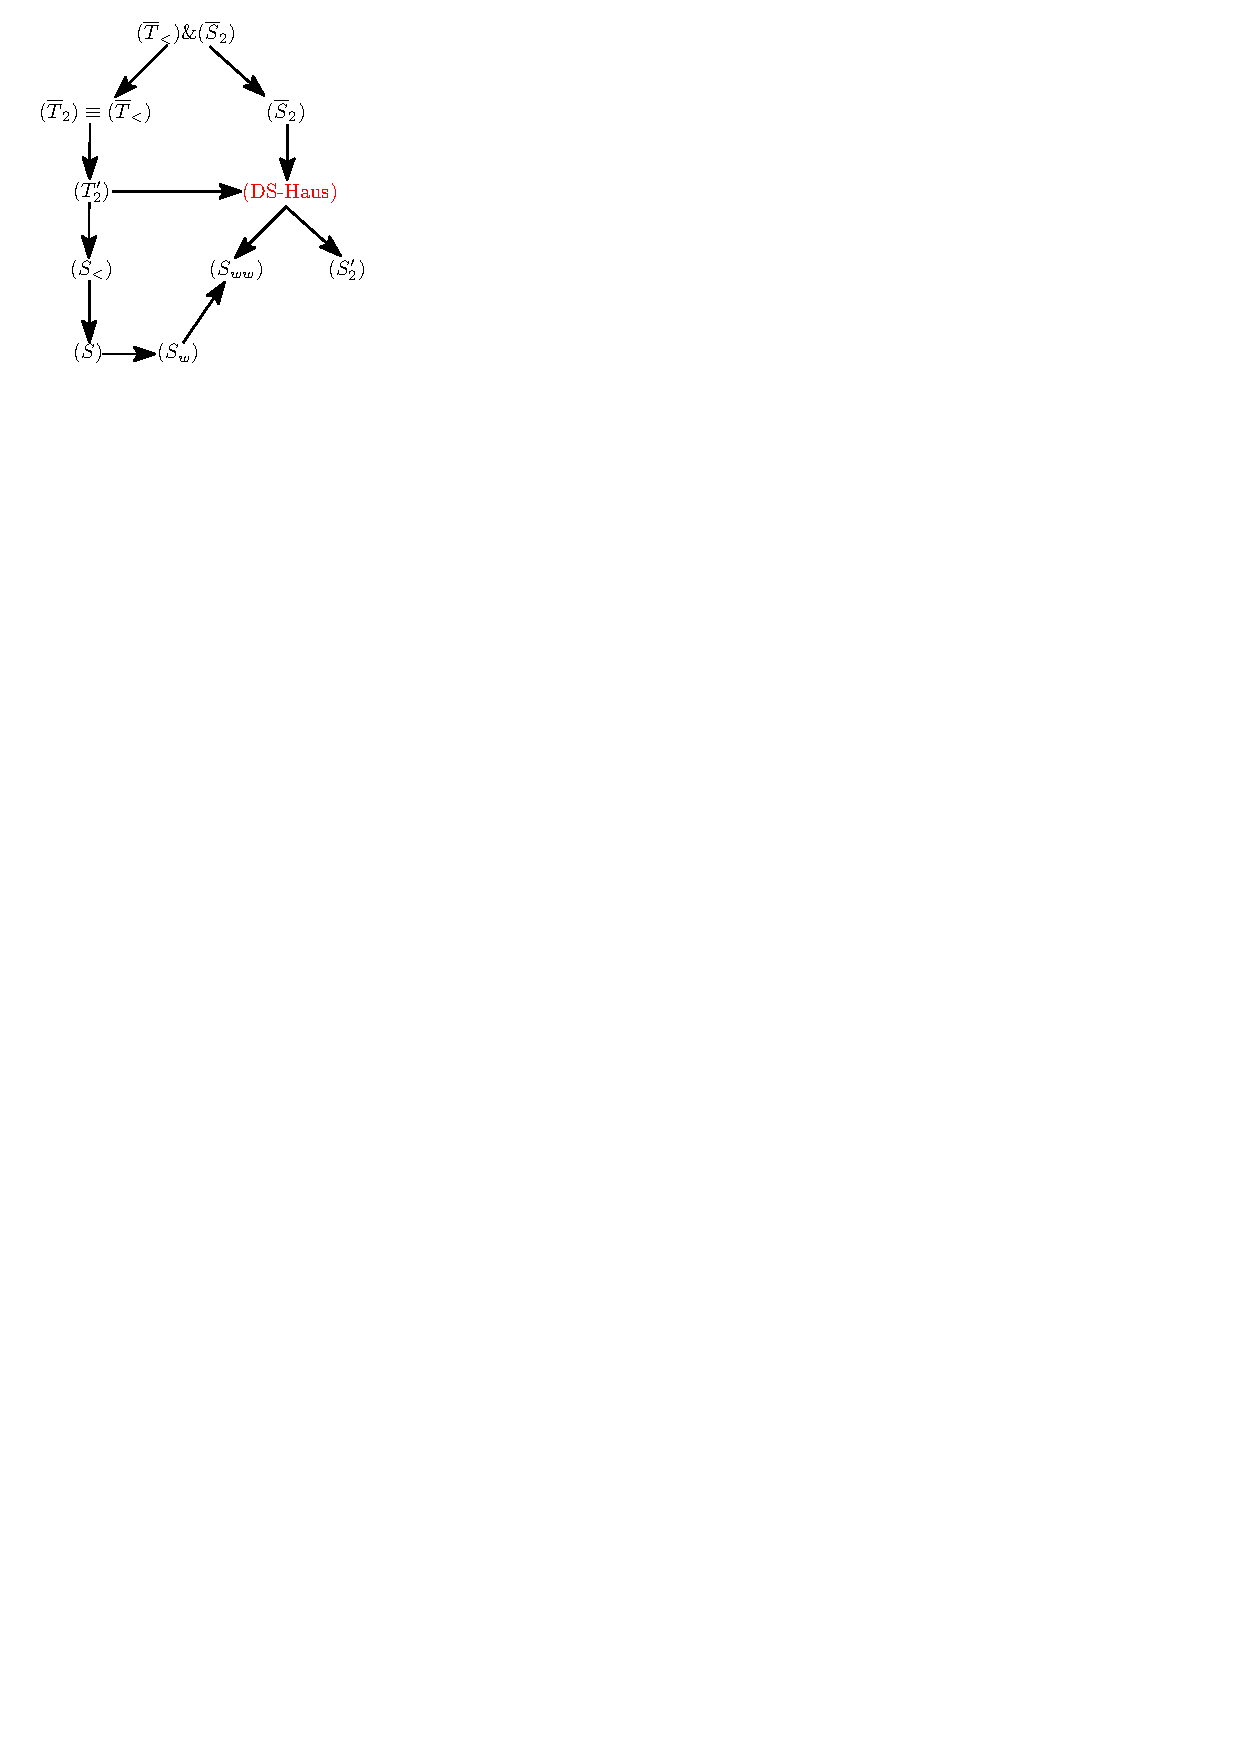
\includegraphics[height=.8\textheight]{img/Hausdorff_diagram.pdf}
\end{figure}
\end{frame}

%------------------------------------------------

\subsection{(Úplná) regularita}

\begin{frame}
\frametitle{Regularita}

\begin{block}{Definice $(T_3)$}
  Pro každé $x$ a každou uzavřenou $A \not\owns x$ existují disjunktní otevřené
  množiny $V_1, V_2$ takové, že $x \in V_1, A \subseteq V_2$.
\end{block}

\begin{figure}
  \includegraphics[width=.5\linewidth]{img/t3.pdf}
\end{figure}
\end{frame}

%------------------------------------------------

\begin{frame}
\frametitle{Úplná regularita}

\newcommand{\I}{\mathbb{I}}
\renewcommand{\phi}{\varphi}
\begin{block}{Definice $(T_{3\frac{1}{2}})$}
  Pro každé $x$ a každou uzavřenou $A \not\owns x$ existuje spojitá funkce 
  $\phi\colon X \to \I$ taková, že
  \begin{enumerate}
    \item $\phi(x) = 0$
    \item $\phi[A] = \{1\}$
  \end{enumerate}
\end{block}

\end{frame}

%------------------------------------------------

\subsection{Normalita}

\begin{frame}
\frametitle{Normalita}
\begin{block}{Definice $(T_4)$}
  Pro každé dvě disjunktní uzavřené $A, B$ existují disjunktní otevřené množiny
  $V_1, V_2$ takové, že $A \subseteq V_1, B \subseteq V_2$.
\end{block}

\begin{figure}
  \includegraphics[width=.5\linewidth]{img/t4.pdf}
\end{figure}

\end{frame}

%------------------------------------------------

\begin{frame}
\frametitle{Multiple Columns}
\begin{columns}[c] % The "c" option specifies centered vertical alignment while the "t" option is used for top vertical alignment

\column{.45\textwidth} % Left column and width
\textbf{Heading}
\begin{enumerate}
\item Statement
\item Explanation
\item Example
\end{enumerate}

\column{.5\textwidth} % Right column and width
Lorem ipsum dolor sit amet, consectetur adipiscing elit. Integer lectus nisl, ultricies in feugiat rutrum, porttitor sit amet augue. Aliquam ut tortor mauris. Sed volutpat ante purus, quis accumsan dolor.

\end{columns}
\end{frame}

%------------------------------------------------
\section{Závěr}
%------------------------------------------------

\begin{frame}
\frametitle{Table}
\begin{table}
\begin{tabular}{l l l}
\toprule
\textbf{Treatments} & \textbf{Response 1} & \textbf{Response 2}\\
\midrule
Treatment 1 & 0.0003262 & 0.562 \\
Treatment 2 & 0.0015681 & 0.910 \\
Treatment 3 & 0.0009271 & 0.296 \\
\bottomrule
\end{tabular}
\caption{Table caption}
\end{table}
\end{frame}

%------------------------------------------------

\begin{frame}
\frametitle{Theorem}
\begin{theorem}[Mass--energy equivalence]
$E = mc^2$
\end{theorem}
\end{frame}

%------------------------------------------------

\begin{frame}[fragile] % Need to use the fragile option when verbatim is used in the slide
\frametitle{Verbatim}
\begin{example}[Theorem Slide Code]
\begin{verbatim}
\begin{frame}
\frametitle{Theorem}
\begin{theorem}[Mass--energy equivalence]
$E = mc^2$
\end{theorem}
\end{frame}\end{verbatim}
\end{example}
\end{frame}

%------------------------------------------------

\begin{frame}
\frametitle{Figure}
Uncomment the code on this slide to include your own image from the same directory as the template .TeX file.
%\begin{figure}
%\includegraphics[width=0.8\linewidth]{test}
%\end{figure}
\end{frame}

%------------------------------------------------

\begin{frame}[fragile] % Need to use the fragile option when verbatim is used in the slide
\frametitle{Citation}
An example of the \verb|\cite| command to cite within the presentation:\\~

This statement requires citation \cite{p1}.
\end{frame}

%------------------------------------------------

\begin{frame}
\frametitle{References}
\footnotesize{
\begin{thebibliography}{99} % Beamer does not support BibTeX so references must be inserted manually as below
\bibitem[Smith, 2012]{p1} John Smith (2012)
\newblock Title of the publication
\newblock \emph{Journal Name} 12(3), 45 -- 678.
\end{thebibliography}
}
\end{frame}

%------------------------------------------------

\begin{frame}
\Huge{\centerline{Děkuji}}
\Huge{\centerline{za}}
\Huge{\centerline{pozornost!}}
\end{frame}

%----------------------------------------------------------------------------------------

\end{document} 
